% Created 2018-09-05 Wed 13:02
% Intended LaTeX compiler: pdflatex
\documentclass[11pt]{article}
\usepackage[utf8]{inputenc}
\usepackage[T1]{fontenc}
\usepackage{graphicx}
\usepackage{grffile}
\usepackage{longtable}
\usepackage{wrapfig}
\usepackage{rotating}
\usepackage[normalem]{ulem}
\usepackage{amsmath}
\usepackage{textcomp}
\usepackage{amssymb}
\usepackage{capt-of}
\usepackage{hyperref}
\usepackage[T1]{fontenc}
\usepackage{mathpazo}
\linespread{1.05}
\usepackage[scaled]{helvet}
\usepackage{courier}
\date{\today}
\title{F3OF Modelling Results}
\hypersetup{
 pdfauthor={},
 pdftitle={F3OF Modelling Results},
 pdfkeywords={},
 pdfsubject={},
 pdfcreator={Emacs 25.3.1 (Org mode 9.1.13)}, 
 pdflang={English}}
\begin{document}

\maketitle
\tableofcontents

\clearpage

\section{F3OF System Overview}
\label{sec:org5a1202f}

\begin{figure}[htbp]
\centering
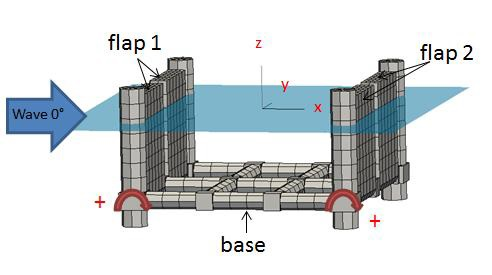
\includegraphics[width=.9\linewidth]{images/system/f3of.jpg}
\caption{\label{fig:org8863164}
Schematic of the F3OF device.}
\end{figure}

Key parameters are taken from \cite{Combourieu2015}  \footnote{N.B. Some parameters given in `InWave - Validation Manual v1.0.0-beta2' differ to the paper.}

\begin{table}[htbp]
\caption{\label{tab:orgbce3e80}
F3OF System - Key Parameters}
\centering
\begin{tabular}{lrrr}
Parameter & Base & Flap 1 & Flap 2\\
\hline
Mass (kg) & 1089825 & 179250 & 179250\\
COG - x (m) & 0 & -12.5 & 12.5\\
COG - y (m) & 0 & 0 & 0\\
COG - z (m) & -9 & -5.5 & -5.5\\
Pitch inertia around body COG (kg.m2) & 76300000 & 1300000 & 1300000\\
Mooring stiffness (N/m) & 100000 & n/a & n/a\\
\end{tabular}
\end{table}

\clearpage
\section{HDB}
\label{sec:org495e0d0}
\subsection{Added Mass}
\label{sec:org7227b48}

\begin{figure}[htbp]
\centering
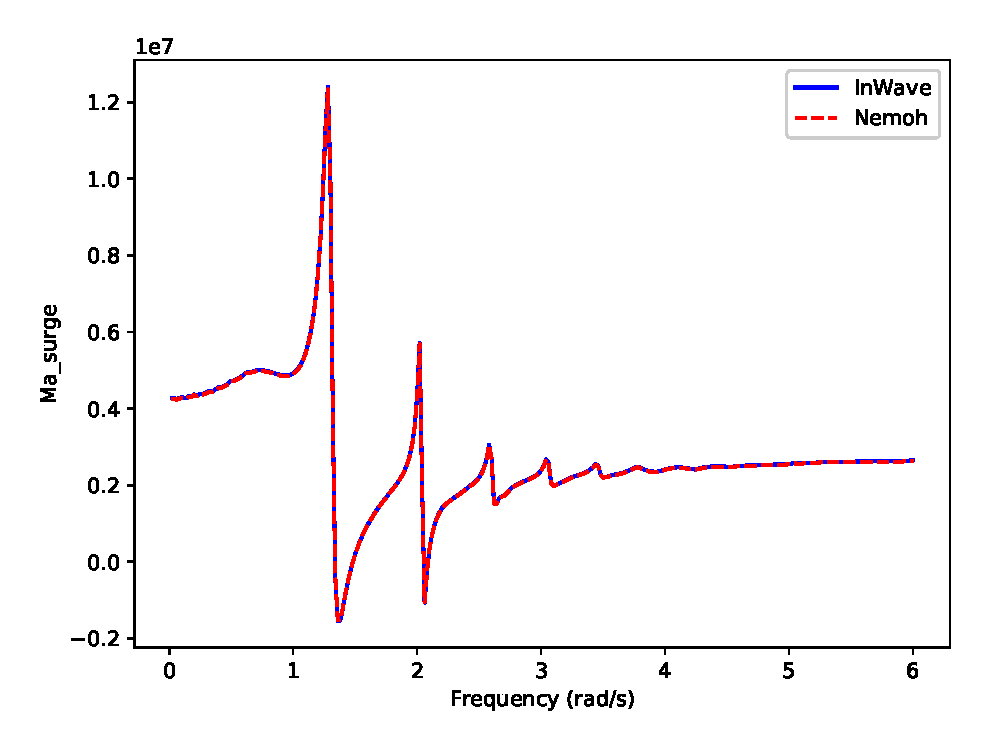
\includegraphics[width=.9\linewidth]{images/hdb/Ma_surge.eps}
\caption{HDB Comparison: Added Mass in Surge Comparison.}
\end{figure}

\begin{figure}[htbp]
\centering
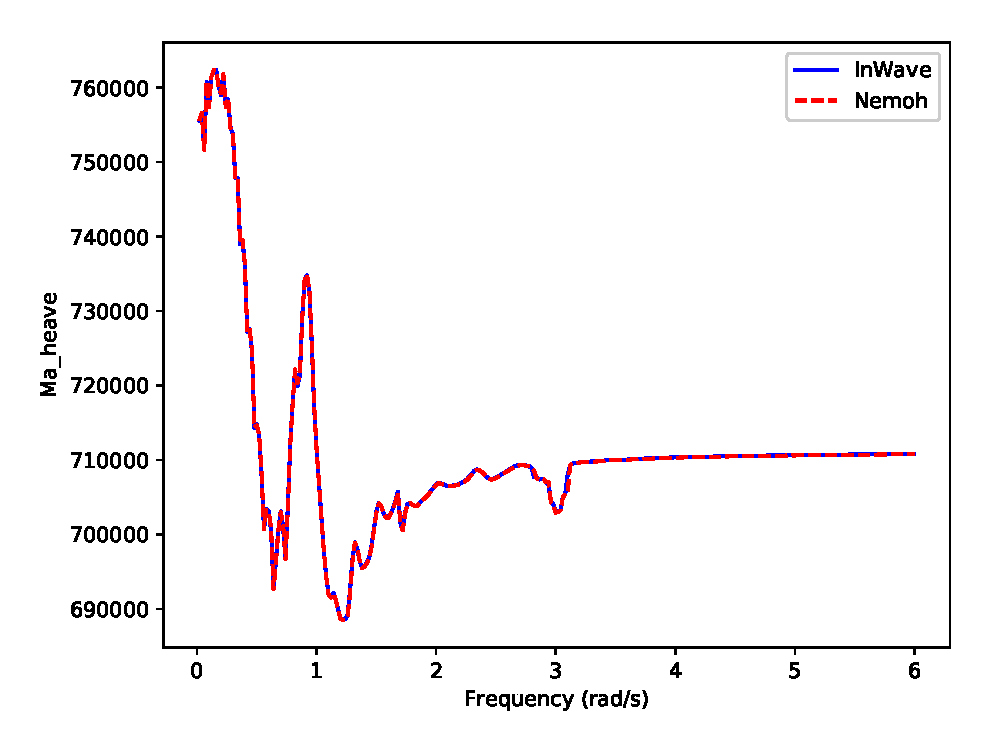
\includegraphics[width=.9\linewidth]{images/hdb/Ma_heave.eps}
\caption{HDB Comparison: Added Mass in Heave Comparison.}
\end{figure}

\begin{figure}[htbp]
\centering
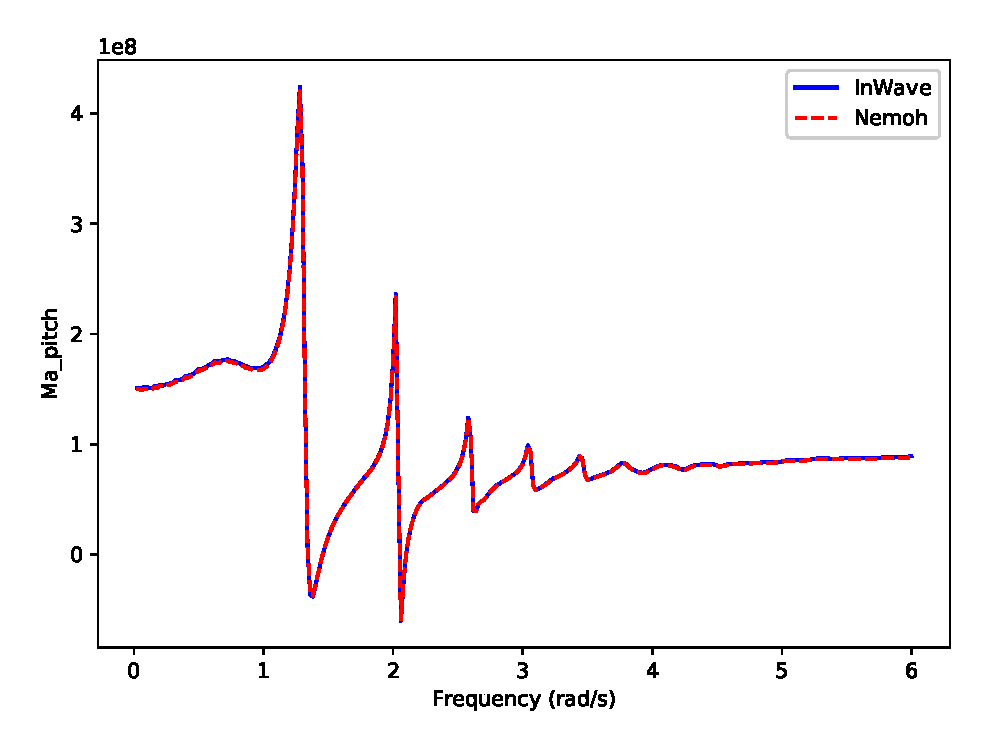
\includegraphics[width=.9\linewidth]{images/hdb/Ma_pitch.eps}
\caption{HDB Comparison: Added Mass in Pitch Comparison.}
\end{figure}

\clearpage
\subsection{Damping}
\label{sec:org89ffc0f}

\begin{figure}[htbp]
\centering
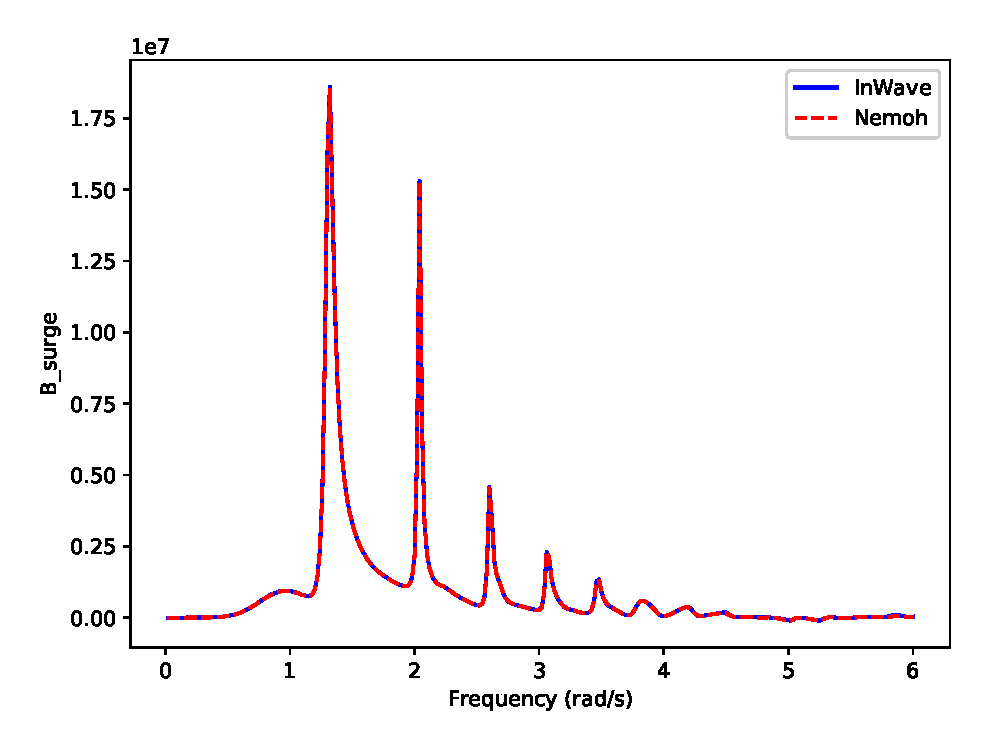
\includegraphics[width=.9\linewidth]{images/hdb/B_surge.eps}
\caption{HDB Comparison: Radiation Damping in Surge.}
\end{figure}

\begin{figure}[htbp]
\centering
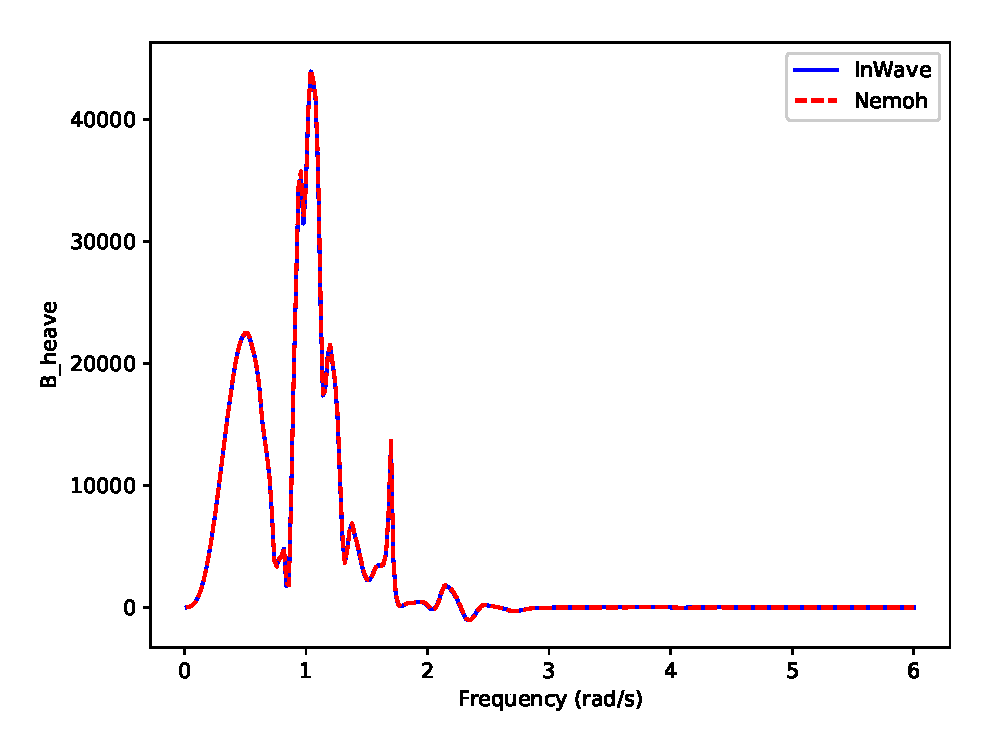
\includegraphics[width=.9\linewidth]{images/hdb/B_heave.eps}
\caption{HDB Comparison: Radiation Damping in Heave.}
\end{figure}

\begin{figure}[htbp]
\centering
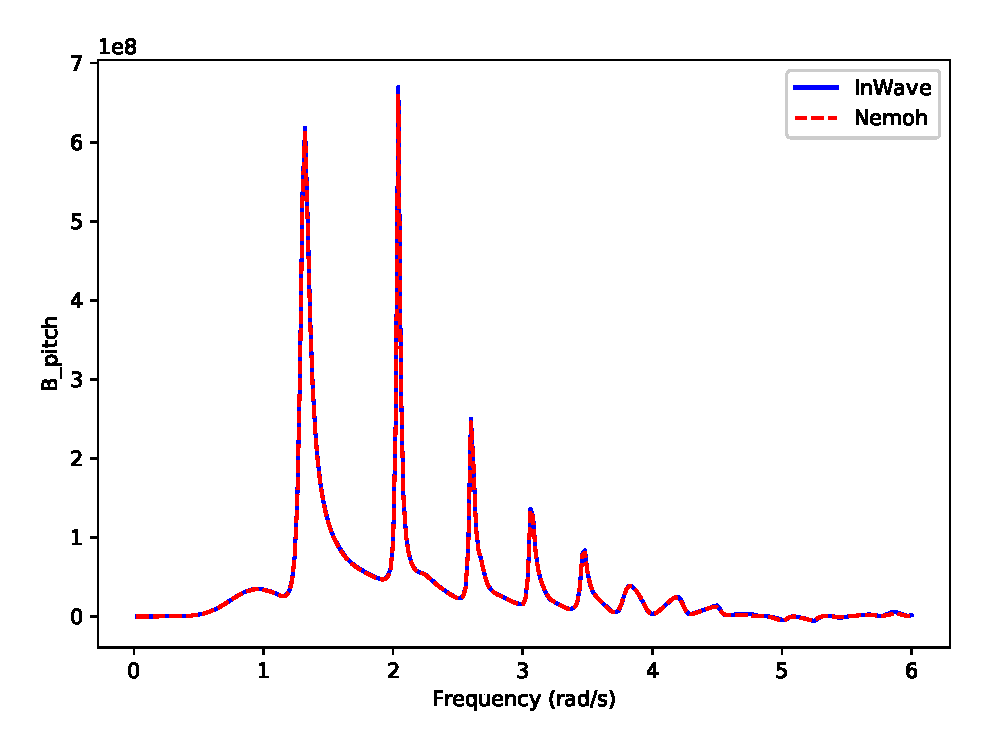
\includegraphics[width=.9\linewidth]{images/hdb/B_pitch.eps}
\caption{HDB Comparison: Radiation Damping in Pitch.}
\end{figure}




\clearpage
\clearpage
\section{Decay Tests}
\label{sec:orgdfa82f3}
\subsection{Initial Position Calculations}
\label{sec:org731c339}
\subsubsection{DT1}
\label{sec:orgc32ec33}

Linear translation:

\begin{equation}
\overrightarrow{p}_{new} = \overrightarrow{p}_{eq} + \overrightarrow{offset}
\end{equation}

Where,

\begin{equation}
\overrightarrow{offset} = \begin{bmatrix} 
                              5\\ 
                              0\\
                              0 
                          \end{bmatrix} m
\end{equation}

\begin{verbatim}
('Base Position : ', [5, 0, -9])
('Flap 1 Position : ', [-7.5, 0.0, -5.5])
('Flap 2 Position : ', [17.5, 0.0, -5.5])
\end{verbatim}

\begin{figure}[htbp]
\centering
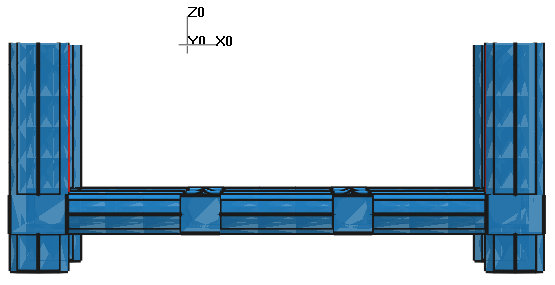
\includegraphics[width=.9\linewidth]{images/system/dt1.png}
\caption{\label{fig:org99e9384}
DT1: Initial position.}
\end{figure}

\newpage
\subsubsection{DT2}
\label{sec:orge230bac}

Rotate whole system by 10 degrees (about the y axis of the base).

\begin{verbatim}
('DT2 Base Position : ', [0.0, 0.0, -9.0])
('DT2 Flap 1 Position : ', [-12.437, 0.0, -5.282])
('DT2 Flap 2 Position : ', [12.559, 0.0, -5.719])
\end{verbatim}

\begin{figure}[htbp]
\centering
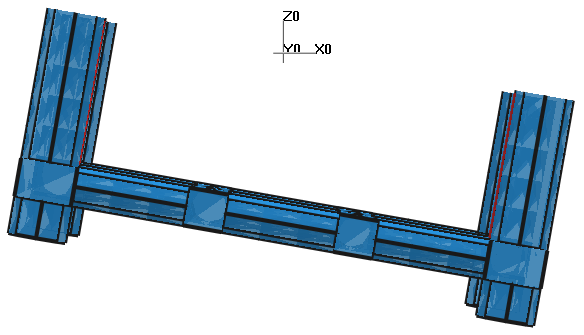
\includegraphics[width=.9\linewidth]{images/system/dt2.png}
\caption{\label{fig:org6aa40c0}
DT2: Initial position.}
\end{figure}


\newpage
\subsubsection{DT3}
\label{sec:org8c1320b}

Rotate flap 1 by 10 degrees.

\begin{verbatim}
('DT2 Base Position : ', [0, 0, -9])
('DT2 Flap 1 Position : ', [-11.892, 0.0, -5.553])
('DT2 Flap 2 Position : ', [12.5, 0.0, -5.5])
\end{verbatim}


\begin{figure}[htbp]
\centering
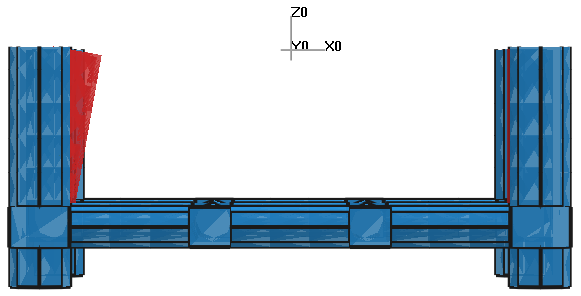
\includegraphics[width=.9\linewidth]{images/system/dt3.png}
\caption{\label{fig:org54dce10}
DT3: Initial position.}
\end{figure}



\newpage





\clearpage
\clearpage
\section{Time Domain Comparison}
\label{sec:org0e95c37}
\subsection{Decay Tests}
\label{sec:orgcf6146f}
\subsubsection{DT1}
\label{sec:orge5c01d0}
\begin{figure}[htbp]
\centering
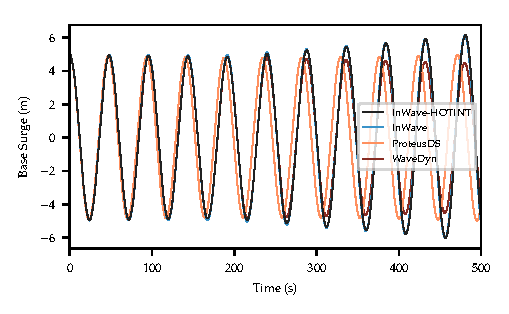
\includegraphics[width=.9\linewidth]{images/dt/DT1_SURGE.pdf}
\caption{Decay Tests: DT1 Surge Comparison.}
\end{figure}

\clearpage
\subsubsection{DT2}
\label{sec:org6f61678}
\begin{figure}[htbp]
\centering
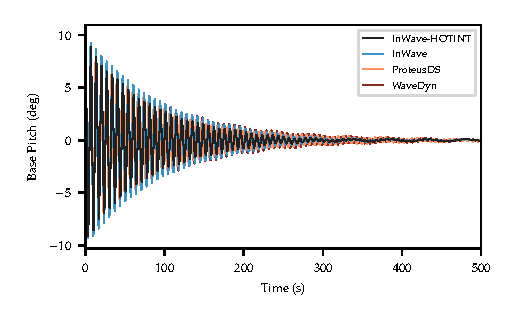
\includegraphics[width=.9\linewidth]{images/dt/DT2_PITCH.pdf}
\caption{Decay Tests: DT2 Pitch Comparison.}
\end{figure}

\begin{figure}[htbp]
\centering
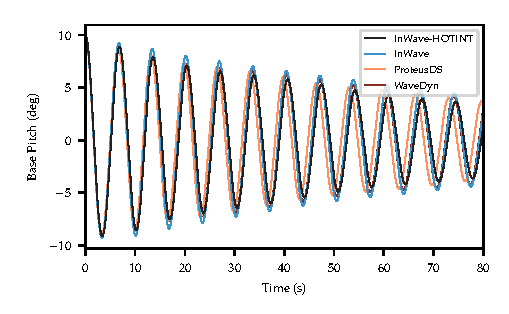
\includegraphics[width=.9\linewidth]{images/dtzoom/DT2_PITCH.pdf}
\caption{Decay Tests: DT2 Pitch Comparison (zoomed).}
\end{figure}


\clearpage
\subsubsection{DT3}
\label{sec:org39f9777}
\begin{figure}[htbp]
\centering
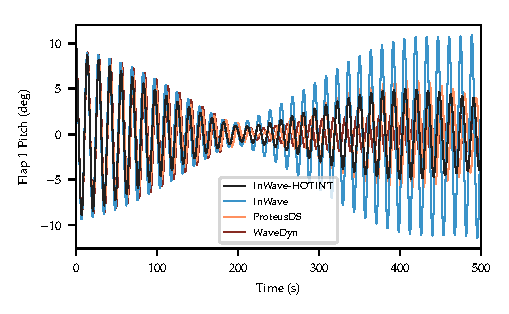
\includegraphics[width=.9\linewidth]{images/dt/DT3_FLAP1.pdf}
\caption{Decay Tests: DT3 Flap 1 Pitch Comparison.}
\end{figure}

\begin{figure}[htbp]
\centering
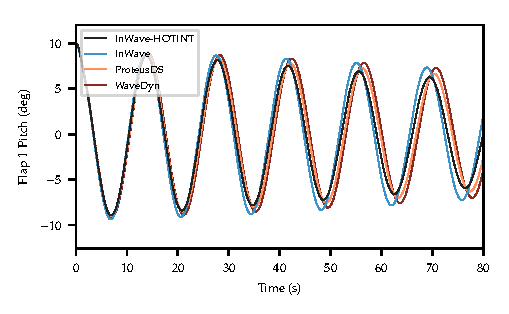
\includegraphics[width=.9\linewidth]{images/dtzoom/DT3_FLAP1.pdf}
\caption{Decay Tests: DT3 Flap 1 Pitch Comparison (zoomed).}
\end{figure}

\begin{figure}[htbp]
\centering
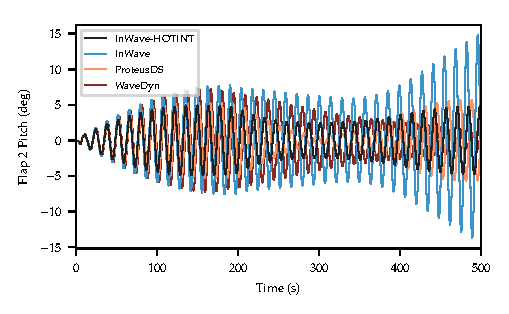
\includegraphics[width=.9\linewidth]{images/dt/DT3_FLAP2.pdf}
\caption{Decay Tests: DT3 Flap 2 Pitch Comparison.}
\end{figure}

\begin{figure}[htbp]
\centering
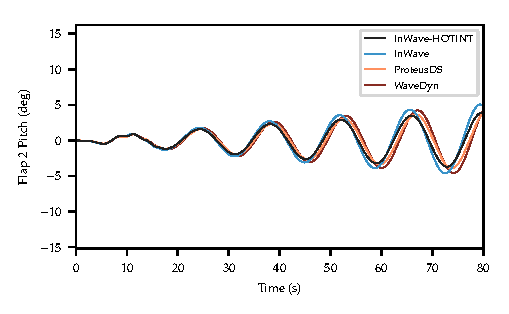
\includegraphics[width=.9\linewidth]{images/dtzoom/DT3_FLAP2.pdf}
\caption{Decay Tests: DT3 Flap 2 Pitch Comparison (zoomed).}
\end{figure}



\clearpage
\section{RAOs}
\label{sec:orgd3c8058}
\subsection{Surge RAO}
\label{sec:org1b17e99}
\begin{figure}[htbp]
\centering
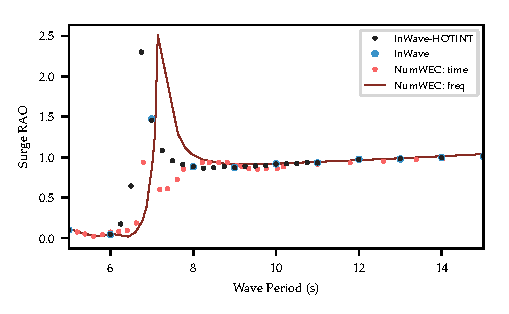
\includegraphics[width=.9\linewidth]{images/rao/rao_surge.pdf}
\caption{Surge RAO Comparison.}
\end{figure}

\clearpage
\subsection{Heave RAO}
\label{sec:org388de5b}
\begin{figure}[htbp]
\centering

\includegraphics[width=.9\linewidth]{images/rao/rao_heave.pdf}
\caption{Heave RAO Comparison.}
\end{figure}

\clearpage
\subsection{Pitch RAO}
\label{sec:org04f3989}
\begin{figure}[htbp]
\centering
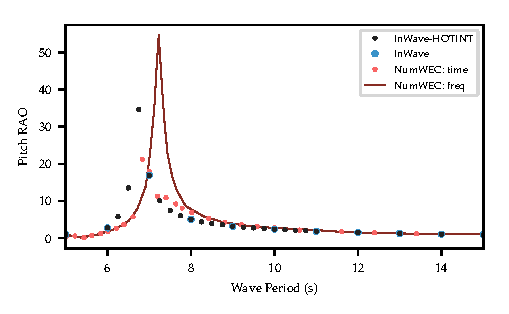
\includegraphics[width=.9\linewidth]{images/rao/rao_pitch.pdf}
\caption{Pitch RAO Comparison.}
\end{figure}
\end{document}